% !TEX root = ../../main.tex

\section{Comparaison des deux résolutions hybrides}
\label{s:compare}

Dans cette section on s'intéressera à la comparaison des méthodes de simulation présentées dans la section~\ref{s:scheme} pour approcher numériquement le modèle VHL. On étudiera en particulier les méthodes de pas de temps adaptatif associées. Nous utilisons dans cette section la condition initiale suivante :
$$
  \begin{aligned}
    u_c(x)   &= 0 \\
    f_h(x,v) &=  \left(\mathcal{M}_{^\alpha/_2,v_0,1}(v) +  \mathcal{M}_{^\alpha/_2,-v_0,1}(v) \right)(1 + \epsilon\cos(kx))
  \end{aligned}
$$
avec $k=0.5$, $\alpha=0.2$, $v_0 = 3.4$, $x\in [0,L]$, $L=4\pi$, $v\in[-12,12]$, et la perturbation $\epsilon = 10^{-2}$. Le champ électrique initial $E(t=0,x)$ est obtenu en résolvant l'équation de Poisson sur notre condition initiale, comme indiqué dans la proposition~\ref{p:vhl_conservation}~:
$$
  \partial_x E(t=0) = (1-\alpha) + \int (1+\epsilon\cos(kx))\left( \mathcal{M}_{^\alpha/_2,v_0,1}(v) + \mathcal{M}_{^\alpha/_2,-v_0,1}(v) \right)\,\mathrm{d}v - 1
$$
La discrétisation du domaine s'effectue avec $N_x=27$ dans la direction $x$, et $N_v=128$ points dans la direction $v$.

Nous allons effectuer deux types de comparaisons entre les méthodes de \emph{splitting} hamiltonien et de Lawson : une comparaison à pas de temps fixe, où on illustrera l'absence de condition de CFL des méthodes de \emph{splitting} ; puis une comparaison des méthodes de pas de temps adaptatif présentées dans la section~\ref{ssec:dtadapt} avec une tolérance $tol = 2\times10^{-5}$.

\subsection{Comparaison des deux résolutions hybrides à pas de temps fixe}

Cette section est dédiée à la comparaison entre la méthode de \emph{splitting} hamiltonien, présentée dans la sous-section~\ref{ssec:splitting}, et la méthode de Lawson présentée dans la sous-section~\ref{ssec:lawson}, pour la résolution du modèle hybride linéarisé~\eqref{eq:vahl}.

Nous considèrerons trois pas de temps différents :
\begin{itemize}
  \item $\Delta t = 0.1 \approx 0.5\Delta v$, il s'agit d'une condition de CFL classique pour des méthodes de volumes finis ;
  \item $\Delta t = 0.5 \approx \sigma\frac{\Delta v}{\|E^n\|_\infty} = 0.54$, with $\sigma\approx 1.732$, il s'agit de la condition de CFL entre WENO5 et RK($4$,$4$) calculée dans le chapitre précédent ou~\cite{Crouseilles:2019b}, et calculée à partir d'une précédente estimation numérique $\|E^n\|_\infty = \max_{i,n}|E^n_i|\approx 0.6$ ;
  \item $\Delta t = 0.7$, il s'agit dans ce cas d'un cas test avec un pas de temps plus grand que la CFL de la méthode de Lawson, pour illustrer que la méthode de \emph{splitting} n'a pas de contrainte de stabilité sur le pas de temps.
\end{itemize}

Sur la figure~\ref{fig:compare:ee}, on trace l'évolution de l'énergie électrique (en échelle semi-log) calculée par deux méthodes d'ordre 4 (méthode de Suzuki et de Lawson-RK(4,4)), avec différentes valeurs de pas de temps $\Delta t$, $0.1$, $0.5$ et $0.7$. On note que toutes les simulations capturent correctement l'énergie électrique dans la phase linéaire, jusqu'au temps 60, même lorsque la méthode est instable. Pour $\Delta t=0.1,0.5$, on vérifie la stabilité prévue des méthodes, qui donnent des résultats très similaires. Dans le cas $\Delta t=0.7$, la méthode de Lawson-RK(4,4) devient instable dans la phase non-linéaire, c'est en fait dans cette phase que l'amplitude du champ électrique atteint son maximum, et le paramètre $\Delta t=0.7$ viole la condition de CFL, alors que la méthode de \emph{splitting} de Suzuki reste stable comme prévu.

\begin{figure}[h]
  \centering
  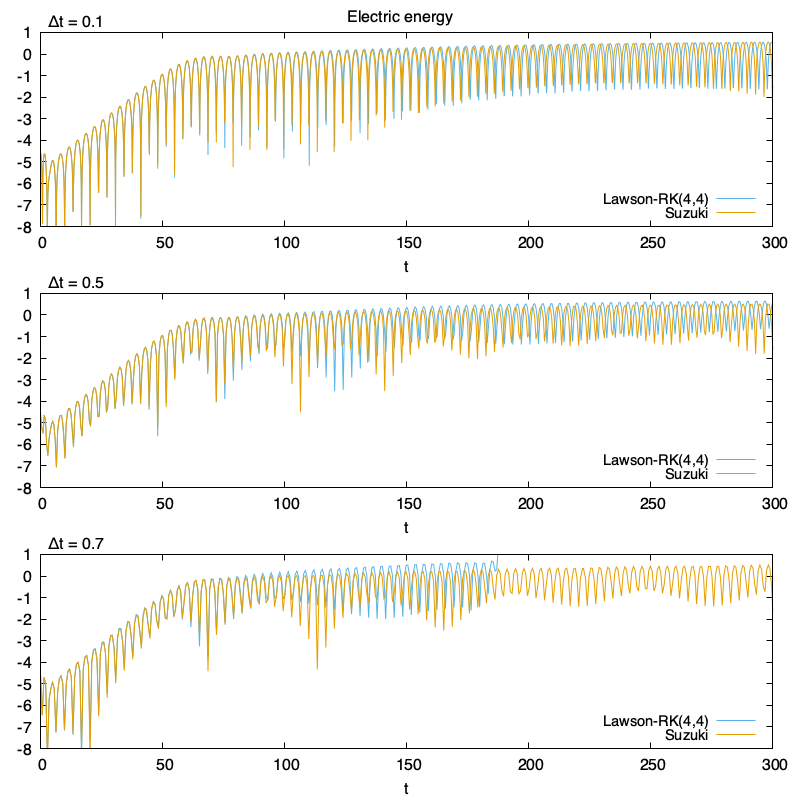
\includegraphics[width=\textwidth]{\localPath/figures/ee_t2.png}
  \caption{Évolution de l'énergie électrique pour le modèle hybride (résolu avec la méthode de Lawson et de Suzuki) pour différentes valeurs de pas de temps $\Delta t=0.1,0.5,0.7$.}
  \label{fig:compare:ee}
\end{figure}


Sur la figure~\ref{fig:H:t2}, on observe l'évolution de l'erreur relative sur l'énergie totale, calculée par :
\begin{equation}
	\frac{\mathcal{H}^n}{\mathcal{H}^0}-1
	\label{eq:relativeerror:H}
\end{equation}
avec :
$$
  \mathcal{H}^n = \frac{1}{2}\iint v^2f_h^n\dd{v}\dd{x}
                + \frac{1}{2}\int\rho_c^{(0)}\left(u_c^n\right)^2\dd{x}
                + \frac{1}{2}\int\left(E^n\right)^2\dd{x}.
$$
On considère les mêmes paramètres numériques et on compare l'effet de la méthode d'intégration en temps (méthode de \emph{splitting} hamiltonien : Lie~\eqref{eq:lie}, Strang~\eqref{eq:strang} et Suzuki~\eqref{eq:suzuki}, et la méthode Lawson-RK(4,4)) sur la préservation de l'énergie totale. On observe que les méthodes géométriques de \emph{splitting} hamiltonien préservent très bien l'énergie totale ; en particulier, l'erreur relative oscille autour d'une constante en temps long, ce qui est un comportement typique d'une méthode géométrique. On observe que la méthode de Lawson que si le pas de temps est pris sous la condition de CFL, l'erreur est proche de $4\%$, ce qui est acceptable. Évidemment, comme évoqué précédemment sur l'énergie électrique, on observe un problème lorsque $\Delta t=0.7$, l'erreur donnée par la méthode Lawson-RK($4$,$4$) diverge dans la phase non-linéaire, à cause de l'instabilité numérique ; avant cela, l'erreur est autour des $2\%$. Le tableau~\ref{tab:H:max} résume le maximum de l'erreur relative $\max_n \left| {\cal H}^n / {\cal H}^0 -1 \right|$ pour les différentes méthodes et les différents pas de temps considérés.

\begin{figure}[h]
  \centering
  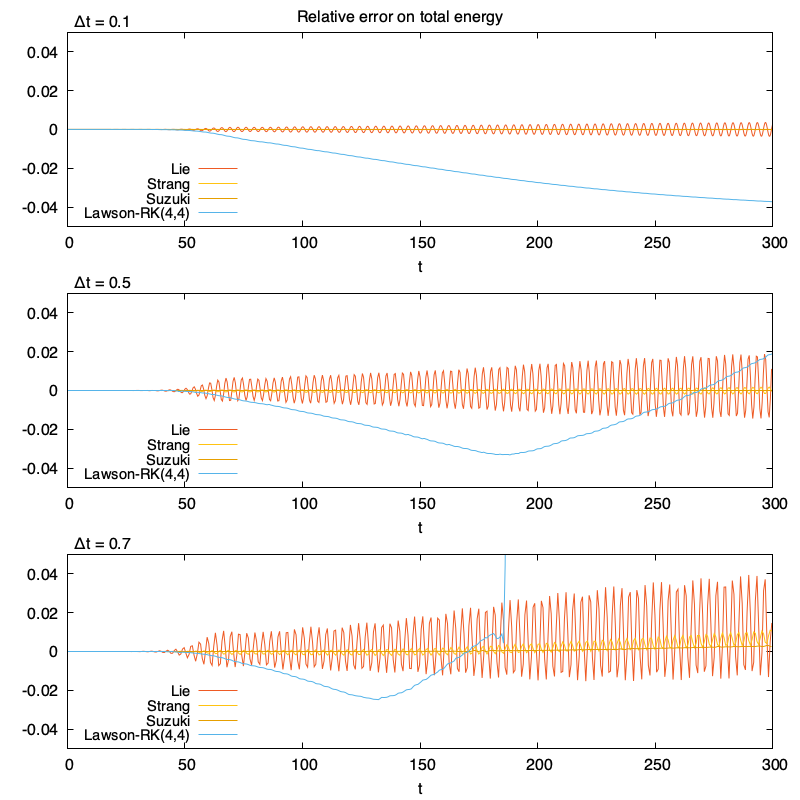
\includegraphics[width=\textwidth]{\localPath/figures/H_t2.png}
  \caption{Évolution de l'erreur relative sur l'énergie totale pour le modèle hybride (résolu avec la méthode de Lawson et de Suzuki) pour différentes valeurs de pas de temps $\Delta t=0.1,0.5,0.7$.}
  \label{fig:H:t2}
\end{figure}

\begin{table}[h]
  \centering
  \begin{tabular}{l|c|c|c}
                   & $0.1$             & $0.5$     & $0.7$        \\
    \hline
    Lie            & $0.0036$          & $0.0187$  & $0.0394$     \\
    Strang         & $0.0001$          & $0.0019$  & $0.0109$     \\
    Suzuki         & $3\times 10^{-8}$ & $0.0001$  & $0.0028$     \\
    Lawson-RK(4,4) & $0.0372$          & $0.0331$  & \texttt{NaN} \\
  \end{tabular}
  \caption{Maximum de l'erreur relative donné sur la figure~\ref{fig:H:t2}.}
  \label{tab:H:max}
\end{table}

Dans le cas $\Delta t=0.1$, on compare sur la figure~\ref{fig:vp:t2} la distribution de particules chaudes $f_h$ calculée par les méthodes de Suzuki et de Lawson-RK(4,4) au temps $t=100$, sur laquelle on ajoute la vitesse moyenne des particules froides $u_c$. Les solutions numériques ainsi obtenues sont très proches, la position des vortex et l'allure de la vitesse moyenne des particules froides sont très similaires entre les deux méthodes. On observe aussi que la méthode Lawson-RK(4,4) introduit plus de diffusion numérique que la méthode de Suzuki ; en effet les vortex semblent avoir une meilleure résolution. Cela peut s'expliquer par la discrétisation dans l'espace des phases dans la direction $v$. Avec la méthode de Lawson RK(4,4) nous utilisons une méthode WENO5 (avec limiteurs de pente) ; alors qu'une interpolation d'ordre 5 par des polynômes de Lagrange (sans limiteurs de pente) est utilisée avec la méthode de Suzuki.

\begin{figure}[h]
  \centering
  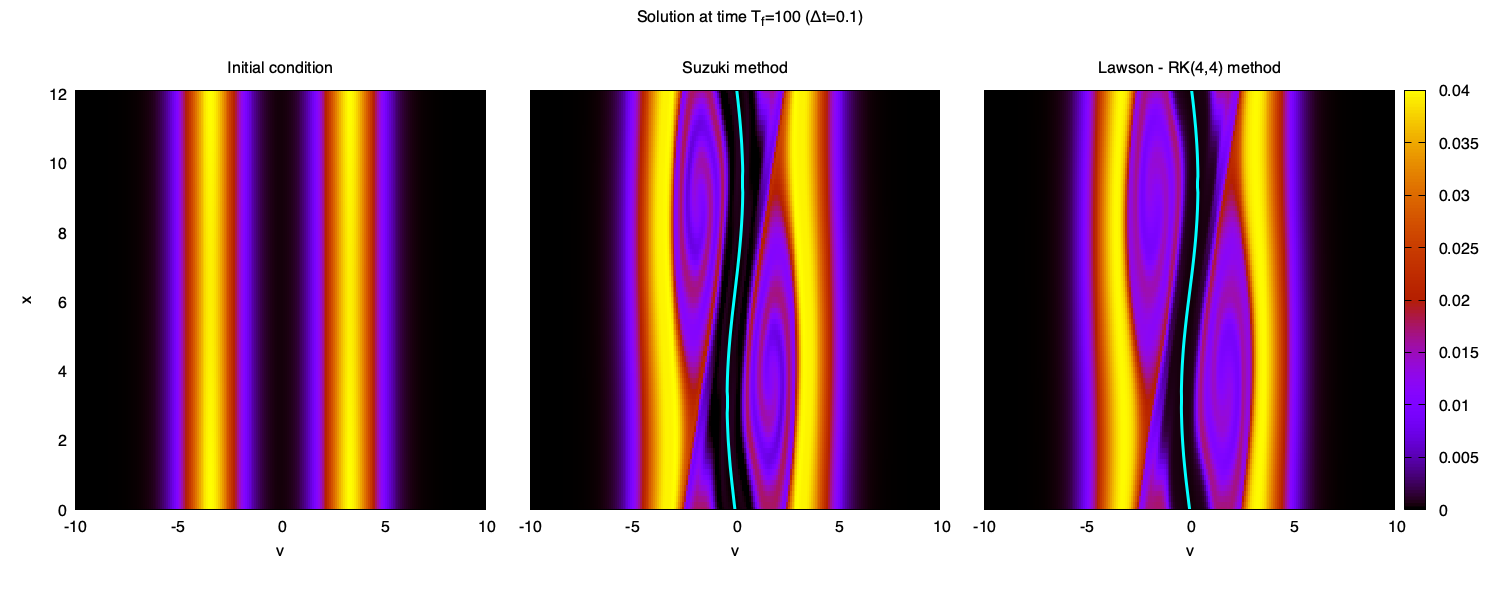
\includegraphics[width=0.9\textwidth]{\localPath/figures/vp_t2.png}
  \caption{Densité des particules chaudes $f_h$ et vitesse moyenne des particules froides $u_c$ (en cyan) la condition initiale (gauche), au temps $t=100$ calculée par la méthode de Suzuki (milieu) et calculée par la méthode de Lawson-RK(4,4) (droite).}
  \label{fig:vp:t2}
\end{figure}

\begin{figure}
	\centering
	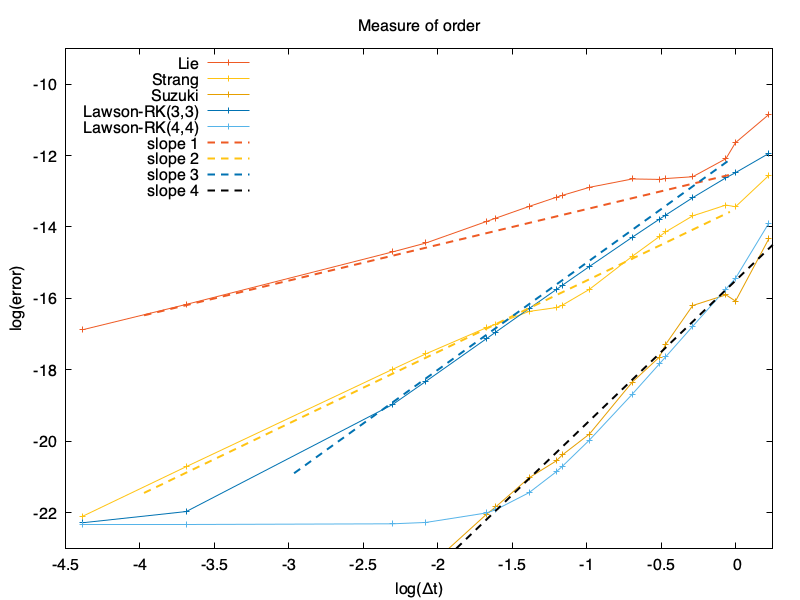
\includegraphics[width=0.75\textwidth]{\localPath/figures/order_t2.png}
	\caption{Étude de l'ordre en temps des différentes méthodes numériques pour résoudre le modèle hybride (méthodes de Lawson et de \emph{splitting}). L'erreur est calculée à partir du maximum de l'erreur relative sur l'énergie totale.}
	\label{fig:order:t2}
\end{figure}

Pour compléter cette étude, on trace sur la figure~\ref{fig:order:t2} l'ordre en temps des différents intégrateurs en temps utilisés pour résoudre le modèle hybride : les méthodes de \emph{splitting} hamiltonien (Lie, Strang et Suzuki), les méthodes de Lawson (RK(4,4) et RK(3,3)). Pour cela on calcule le maximum de l'erreur relative sur l'énergie totale : $\max_n|\mathcal{H}^n/\mathcal{H}^0-1|$, jusqu'au temps $t=15$, en fonction du pas de temps $\Delta t\in[0.01,0.125]$, avec $N_x=243$ et $N_v=512$. Tous les ordres théoriques des méthodes en temps sont bien reconstruits. On remarque que la constante d'erreur entre la méthode de Suzuki et de Lawson-RK(4,4) sont très proches, mais que cette première est légèrement plus coûteuse que la méthode de Lawson (plus de détails dans la section~\ref{ssec:2:time}).

\FloatBarrier

\subsection{Comparaison des deux méthodes de pas de temps adaptatif}
\label{ssec:2:dtn}

Cette section est dédiée à l'étude des méthodes de Suzuki et de Lawson avec leur stratégie de pas de temps adaptatif associée, présentée dans la section~\ref{ssec:dtadapt}. Pour toutes les simulations nous nous sommes intéressés à l'estimateur d'erreur qui dans ce cas s'écrit :
\begin{equation}
  \begin{aligned}
    L^{n+1}_{[3]} & = \left(\sum_{i=0}^{N_x-1}\left( {u_c}_i^{n_1,[4]}-{u_c}_i^{n_1,[3]} \right)^2\Delta x\right)^{\frac{1}{2}}
                    + \left(\sum_{i=0}^{N_x-1}\left( {E}_i^{n_1,[4]}-{E}_i^{n_1,[3]} \right)^2\Delta x\right)^{\frac{1}{2}} \\
                  & + \left(\sum_{i=0}^{N_x-1}\sum_{j=0}^{N_v-1}\left| {f_h}_{i,j}^{n_1,[4]}-{f_h}_{i,j}^{n_1,[3]} \right|^2\Delta v\Delta x\right)^{\frac{1}{2}} \\
                  & = L_{u_c}^{n+1} + L_{E}^{n+1} + L_{f_h}^{n+1},
  \end{aligned}
  \label{eq:LucEfh:localerror}
\end{equation}
où ${u_c}_i^{n+1,[p]}$,${E}_i^{n+1,[p]}$ et ${f_h}_{i,j}^{n+1,[p]}$ sont les inconnues discrétisées calculées avec une méthode d'ordre $p$ en temps et associées au temps $t^{n+1}$ et au point $x_i=i\Delta x$, $i=0,\dots,N_x$ et $v_j = -v_\text{max} + j\Delta v$, $j=0,\dots,N_v$ de l'espace des phases. Pour les deux méthodes, si le critère d'erreur $\|L_{[3]}^{n+1}\|<tol$ est satisfait, alors l'itération est acceptée et le temps incrémenté, sinon l'itération est rejetée et reprend au temps $t^n$. Dans les deux cas, le pas de temps suivant est calculé en utilisant~\eqref{eq:dtopt}. Cela nous permet de comparer l'estimateur d'erreur avec la même tolérance $tol$ (prise arbitrairement à $tol=2\times10^{-5}$) entre les deux intégrateurs en temps : la méthode de Suzuki et DP4(3). Nous regarderons aussi la taille des pas de temps proposés par les deux méthodes et le nombre d'itérations nécessaires pour finir la simulation.

\begin{table}[h]
	\centering
	\begin{tabular}{c|c|c|c}
      méthode             & nombre d'itérations & nombre d'itérations acceptées & ratio \\
%      \hline
%       $\Delta t = 0.5$ & 600                  & 600                          & 1     \\
%       $\Delta t = 0.1$ & 3000                 & 3000                         & 1     \\
      \hline
      Suzuki              & 23895                & 23849                        & 0.998 \\
      Lawson-DP4(3)       & 2288                 & 2192                         & 0.958 \\
	\end{tabular}
	\caption{Comparaison du nombre d'itérations pour résoudre le problème jusqu'au temps $t=300$, le nombre d'itérations acceptées de la méthode de pas de temps adaptatif et le ratio entre le nombre d'itérations acceptées et le nombre total d'itérations.}
	\label{tab:compare:iteration}
\end{table}

Le tableau~\ref{tab:compare:iteration} présente le nombre d'itérations nécessaires pour atteindre le temps final $t=300$ pour les deux méthodes de pas de temps adaptatif considérées (méthode de Suzuki et de Lawson-DP4(3)) avec les paramètres numériques suivants $N_x=81$, $N_v=128$. Le nombre d'itérations acceptées (itérations où le critère d'erreur $\|L_{[3]}^{n+1}\|<tol$ est satisfait), et le ratio entre le nombre d'itérations acceptées et le nombre total d'itérations sont aussi présentés. On observe qu'une très large majorité des itérations sont acceptées pour les deux méthodes, ce qui signifie que l'estimateur d'erreur est un bon indicateur. Pour la méthode de Lawson-DP4(3) le ratio d'itérations acceptées est légèrement plus faible que pour la méthode de Suzuki, ce qui signifie que la stratégie de pas de temps adaptatif essaie des pas de temps plus larges qui sont parfois rejetés. La très faible proportion d'itérations rejetées indique qu'il est très rarement nécessaire de recalculer une itération avec un pas de temps plus petit. Le surcoût engendré par la méthode de pas de temps adaptatif est donc négligeable. La seconde remarque que l'on peut faire est à propos de la méthode de Suzuki, qui nécessite 10 fois plus d'itérations que la méthode de Lawson-DP4(3) pour atteindre le temps final $t=300$, ce qui signifie que la méthode de Suzuki nécessite de plus petits pas de temps pour satisfaire le critère d'erreur $\|L_{[3]}^{n+1}\|<tol$.

Sur la figure~\ref{fig:compare:dt_and_error} est représentée l'évolution de la taille du pas de temps au cours du temps ; en effet celui-ci suit l'équation~\eqref{eq:dtopt} et est donc recalculé à chaque itération. Les itérations rejetées, celles où le critère d'erreur n'est pas satisfait, sont représentées avec des carrés. On remarque tout d'abord que dans la phase linéaire (jusqu'au temps $t\approx 50$) des pas de temps plus grands sont pris. Pendant la phase non-linéaire, le pas de temps oscille près d'une constante, qui permet de capturer les effets non-linéaires (vortex dans la distribution de particules) et les forts gradients (filamentation issue de la formation des vortex). On remarque ensuite, que pour une même tolérance ($tol=2\times10^{-5}$), la méthode de Suzuki nécessite de plus petits pas de temps, comparée à la méthode DP4(3), pour satisfaire le critère d'erreur, comme remarqué dans le tableau~\ref{tab:compare:iteration}. On remarque que les variations du pas de temps sont relativement importantes ; il est possible de contrôler ces oscillations en limitant l'évolution des pas de temps, en prenant par exemple $\Delta t^{n+1}\in[0.5\Delta t^n,2\Delta t^n]$, comme proposé dans \cite{Balac:2014}. Sur la figure~\ref{fig:compare:error:dtc} est tracée l'évolution de l'erreur locale $L_{[3]}^n$ comme une fonction du temps pour la méthode de Lawson (gauche) et de Suzuki (droite), avec une stratégie de pas de temps adaptatif et une stratégie de pas de temps constant. Pour un grand pas de temps ($\Delta t = 0.5$), les méthodes sont stables, mais le pas de temps dépasse largement la tolérance fixée à $tol=2\times10^{-5}$. Les méthodes à pas de temps adaptatif choisissent automatiquement un pas de temps permettant de garantir une erreur locale en-dessous de la tolérance.
Les simulations réalisées à partir de la méthode de Lawson avec un pas de temps adaptatif (DP4(3)) et un pas de temps fixe (RK(4,4) avec $\Delta t = 0.1$) donnent une erreur locale très proche. On remarque cependant que la méthode DP4(3) optimise son pas de temps pour assurer une erreur locale sous la tolérance, et permet d'obtenir des pas de temps plus grands que $\Delta t =0.1$, comme on peut le remarquer sur la figure~\ref{fig:compare:dt_and_error}. Assurer une erreur sous une tolérance avec les plus grands pas de temps possibles est une heuristique intéressante. En ce qui concerne les résultats avec la méthode de Suzuki, on remarque de nouveau que la stratégie requiert de plus petits pas de temps, en comparaison avec DP4(3), pour assurer une estimation de l'erreur locale sous la tolérance. De plus, avec un pas de temps constant à $\Delta t = 0.1$, la méthode de Suzuki génère des erreurs locales bien plus importantes, alors que la méthode DP4(3) était presque sous la tolérance.

\begin{figure}[h]
  \centering
  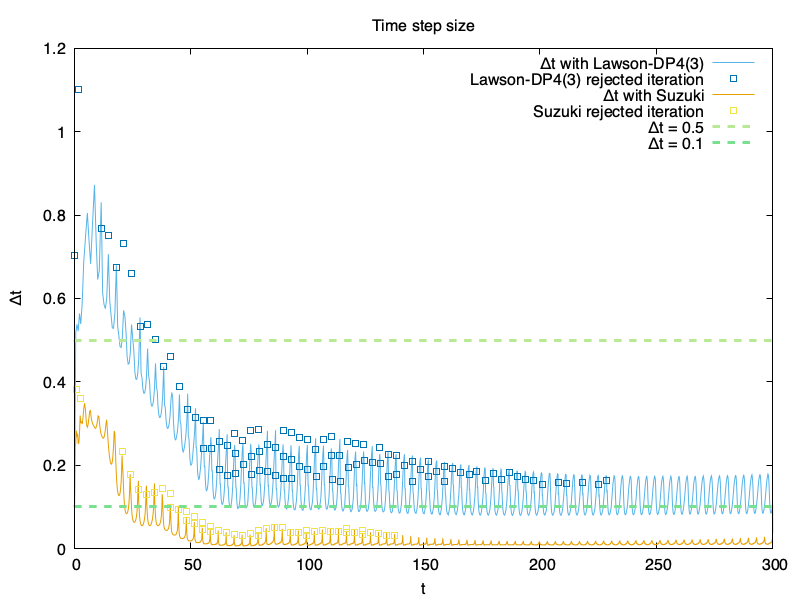
\includegraphics[width=0.75\textwidth]{\localPath/figures/dt_size_t3.png}
  \caption{Évolution du pas de temps $\Delta t_n$ (les itérations rejetées sont représentées par des carrés) pour le modèle hybride avec des méthodes de pas de temps adaptatif.} 
  \label{fig:compare:dt_and_error}
\end{figure}

\begin{figure}[h]
  \centering
  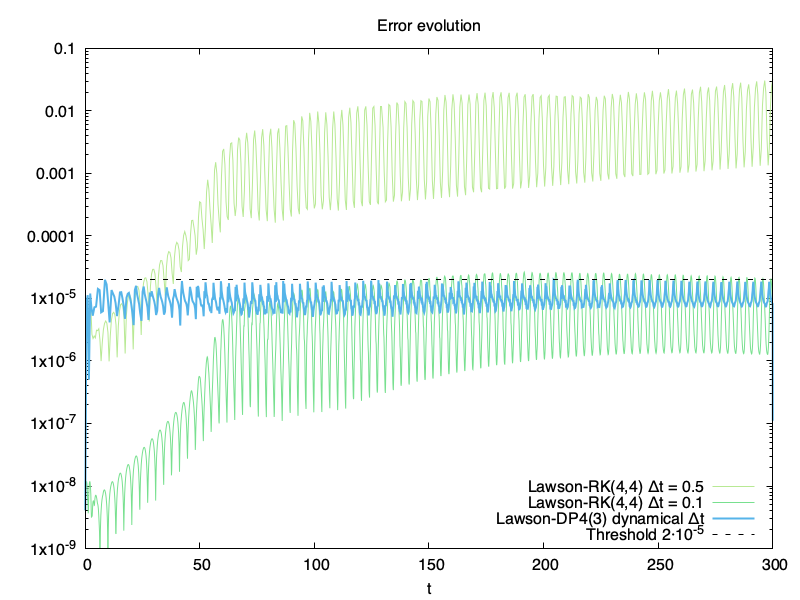
\includegraphics[width=0.49\textwidth]{\localPath/figures/Ll_t3.png}
  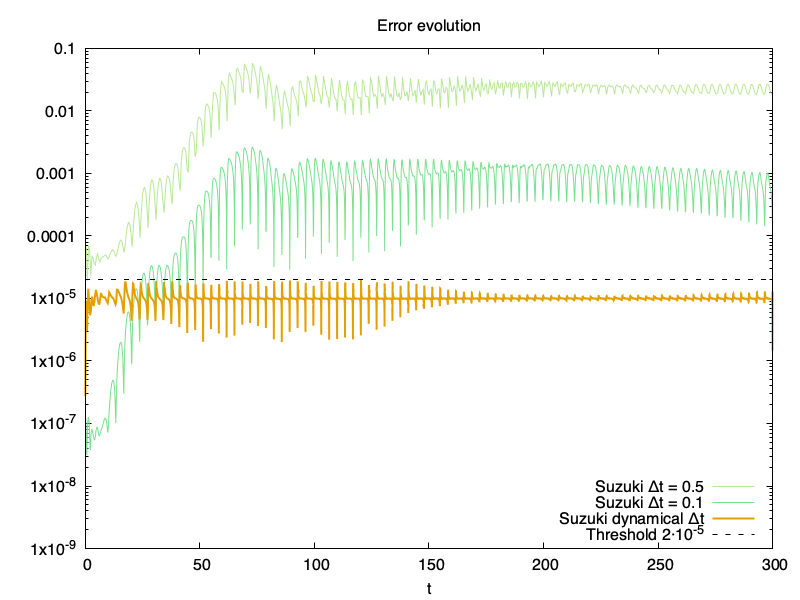
\includegraphics[width=0.49\textwidth]{\localPath/figures/Ls_t3.png}
  \caption{Comparaison de l'évolution en temps de l'estimateur d'erreur pour une méthode à pas de temps constant et à pas de temps adaptatif. La méthode de Lawson est à gauche. La méthode de Suzuki est à droite. Les résultats sont en échelle semi-$\log$.}
  \label{fig:compare:error:dtc}
\end{figure}
\begin{figure}[h]
  \centering
  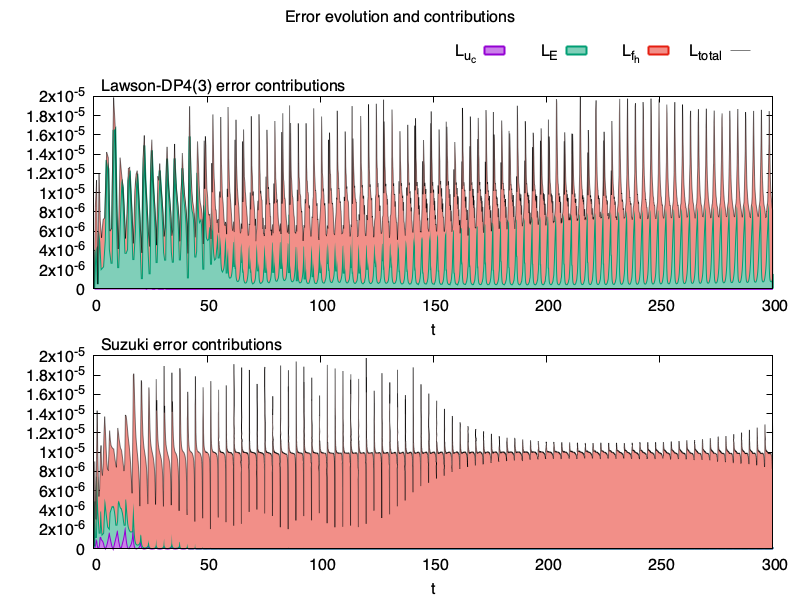
\includegraphics[width=0.8\textwidth]{\localPath/figures/L_LucEfh_t3.png}
  \caption{Comparaison de la contribution de chaque composante de l'estimateur d'erreur locale en fonction du temps, pour la méthode de Lawson (haut) et de Suzuki (bas).}
  \label{fig:compare:error:LucEfh}
\end{figure}

Pour les deux méthodes à pas de temps adaptatif, on s'intéresse maintenant à l'évolution de l'estimateur d'erreur locale au cours du temps, en prenant en compte les différentes contributions de $L^n_{[3]}$, à savoir $L^n_{u_c}$, $L^n_{E}$ et $L^n_{f_h}$ définies dans~\eqref{eq:LucEfh:localerror}. Les résultats sont visibles sur la figure~\ref{fig:compare:error:LucEfh}. L'estimation de l'erreur locale et ses contributions y sont tracées, pour la méthode DP4(3) en haut, et pour la méthode de Suzuki en bas. Pour la méthode DP4(3), on remarque tout d'abord que la contribution venant de $L^n_{u_c}$ est négligeable (autour de l'erreur machine), ce qui peut s'expliquer par le fait que dans la méthode de Lawson la partie linéaire est résolue exactement. Puisque la partie non-linéaire de la méthode de Lawson comprend le calcul du courant chaud $\int vf_h\dd{v}$ qui va impacter $L^n_E$ et le transport dans la direction $v$ qui va impacter $L^n_{f_h}$, les contributions à l'estimateur d'erreur de ces deux contributions restent prépondérantes tout au long de la simulation. Pour la méthode de Suzuki, l'erreur provient essentiellement de $L^n_{f_h}$, erreur venant de l'interpolation du transport dans la direction $v$. Il est à noter, que les erreurs $L^n_{u_c}$, $L^n_{E}$ ne sont pas nulles au delà du temps $t\approx 50$, mais sont respectivement de l'ordre de $10^{-10}$ et $10^{-8}$.

%\FloatBarrier

\subsection{À propos des temps de calcul}
\label{ssec:2:time}

Pour finir la comparaison entre les méthodes de \emph{splitting} et de Lawson, nous comparerons leurs temps de calcul. Sur la figure~\ref{fig:timer_boxplot_t4} (gauche), on représente la valeur moyenne ainsi que les quartiles du temps de calcul d'une itération de RK(4,4), DP4(3) et de la méthode de Suzuki. Nous rappelons que la méthode RK(4,4) est constituée de 4 étages, alors que les méthodes DP4(3) et de Suzuki en comprennent 5. Cela explique pourquoi une itération de la méthode RK(4,4) coûte moins qu'une itération des deux autres méthodes. Sur la partie de droite de la figure~\ref{fig:timer_boxplot_t4} on compare le temps de calcul de chaque étape des différentes méthodes. On rappelle que la méthode DP4(3) est formée à partir des 4 étages de la méthode RK(4,4) plus un étage supplémentaire. Comme espéré, chaque étape de la méthode de Suzuki a le même coût (puisque la méthode de Suzuki est une composition de 5 méthode de Strang). Au contraire, on observe que les deux premiers étages des méthodes RK(4,4) ou DP4(3) sont moins coûteux que les autres étages, ces deux premiers contenant moins d'opérations.

\begin{figure}[h]
  \centering
  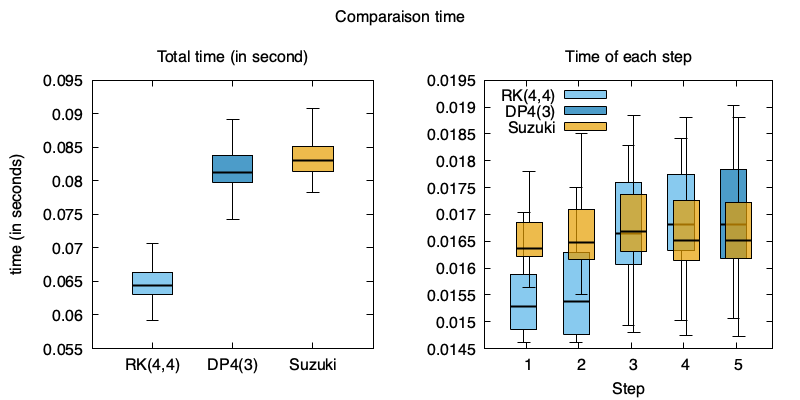
\includegraphics[width=\textwidth]{\localPath/figures/timer_boxplot_t4.png}
  \caption{Valeur moyenne et quartiles du temps de calcul sur une itération (gauche) et pour chaque étape d'une itération (droite).}
  \label{fig:timer_boxplot_t4}
\end{figure}
